% !TEX TS-program = lualatex
% !TEX encoding = UTF-8 Unicode

\documentclass{beamer}

\mode<presentation>
{
  \usetheme{Madrid} % or try Darmstadt, Madrid, Warsaw, ...
  % or ...
  \setbeamertemplate{bibliography item}{}
  \setbeamercovered{transparent}
  % or whatever (possibly just delete it)
}

\usepackage{fontspec}
\usepackage[english]{babel}
% or whatever
\usepackage{csquotes}
\usepackage[backend=biber,
        style=unified,
        maxcitenames=3,
        maxbibnames=99,
        natbib,
        url=false]{biblatex}
% \addbibresource{Dissertation.bib}
\setmainfont{Libertinus Sans} % Main font
% \setsansfont{libertinus sansserif} % Sans serif font
% \setmonofont{CMU Typewriter Text}
\renewcommand{\ttdefault}{cmtt}

% \usepackage[colorlinks,allcolors={black},urlcolor={blue}]{hyperref} %allows for hyperlinks and pdf bookmarks 
\usepackage{graphicx}	%Inserting graphics, pictures, images 		
\usepackage{multicol} %Multicolumn text
\usepackage{multirow} %Useful for combining cells in tablesbrew 
% \usepackage{booktabs} %Enhanced tables
% \usepackage{underscore} %Allows for underscores in text mode
% \usepackage[colorlinks,allcolors={black},urlcolor={blue}]{hyperref} %allows for hyperlinks and pdf bookmarks
\usepackage{url} %allows for urls
\def\UrlBreaks{\do\/\do-} %allows for urls to be broken up
% \usepackage[normalem]{ulem} %strike out text. Handy for syntax
% \usepackage{tcolorbox}
% \usepackage{datetime2}
\usepackage{caption}
\usepackage{subcaption}
\usepackage{langsci-gb4e} % Language Science Press' modification of gb4e
\usepackage{tikz} % Drawing Hasse diagrams
\usetikzlibrary{decorations.pathreplacing}
\usepackage{leipzig} %	Offers support for Leipzig Glossing Rules


\title[LING 450/550] % (optional, use only with long paper titles)
{Introduction to Linguistic Phonetics}

\subtitle{Course Introduction}

\author[Brinkerhoff] % (optional, use only with lots of authors)
{Mykel Loren Brinkerhoff}
% - Give the names in the same order as the appear in the paper.
% - Use the \inst{?} command only if the authors have different
%   affiliation.

\institute[UW] % (optional, but mostly needed)
{University of Washington}
% - Use the \inst command only if there are several affiliations.
% - Keep it simple, no one is interested in your street address.

\date[2025-09-25] % (optional, should be abbreviation of conference name)
{September 25, 2025}
% - Either use conference name or its abbreviation.
% - Not really informative to the audience, more for people (including
%   yourself) who are reading the slides online

% \subject{Theoretical Computer Science}
% This is only inserted into the PDF information catalog. Can be left
% out. 



% If you have a file called "university-logo-filename.xxx", where xxx
% is a graphic format that can be processed by latex or pdflatex,
% resp., then you can add a logo as follows:

% \pgfdeclareimage[height=0.5cm]{university-logo}{university-logo-filename}
% \logo{\pgfuseimage{university-logo}}



% Delete this, if you do not want the table of contents to pop up at
% the beginning of each subsection:
% \AtBeginSubsection[]
% {
%   \begin{frame}<beamer>{Outline}
%     \tableofcontents[currentsection,currentsubsection]
%   \end{frame}
% }


% If you wish to uncover everything in a step-wise fashion, uncomment
% the following command: 

%\beamerdefaultoverlayspecification{<+->}


\begin{document}

\begin{frame}
  \titlepage
\end{frame}

% \begin{frame}{Outline}
%   \tableofcontents
%   % You might wish to add the option [pausesections]
% \end{frame}


% Structuring a talk is a difficult task and the following structure
% may not be suitable. Here are some rules that apply for this
% solution: 

% - Exactly two or three sections (other than the summary).
% - At *most* three subsections per section.
% - Talk about 30s to 2min per frame. So there should be between about
%   15 and 30 frames, all told.

% - A conference audience is likely to know very little of what you
%   are going to talk about. So *simplify*!
% - In a 20min talk, getting the main ideas across is hard
%   enough. Leave out details, even if it means being less precise than
%   you think necessary.
% - If you omit details that are vital to the proof/implementation,
%   just say so once. Everybody will be happy with that.
%-----------------------------------------------------------
\section{What is Phonetics?}
%-----------------------------------------------------------
\begin{frame}{What is Phonetics?}
\begin{block}{Question}
    When you hear the word ``phonetics,'' what comes to mind?
\end{block}
\end{frame}

\begin{frame}{What is Phonetics?}
  \begin{itemize}
    \item <1-> The study of the sounds of human speech
    \item <2-> Involves the production, transmission, and perception of speech sounds
    \item <3-> Key areas of focus include articulatory phonetics, acoustic phonetics, and auditory phonetics, and speech perception
  \end{itemize}
\end{frame}

%-----------------------------------------------------------
\section{Teaching team}
%-----------------------------------------------------------
\begin{frame}{Professor}
    \begin{multicols}{2}
        \begin{description}[font=\bfseries]
            \item[Name:] Mykel Loren Brinkerhoff
            \item[Education:] UCSC (Ph.D., 2025)
            \item[Contact:] \href{mailto:mlbrinke@uw.edu}{mlbrinke@uw.edu}
            \item[Research Interests:] Phonetics, Phonology, Phonology interfaces, fieldwork, endangered languages
        \end{description}
        \columnbreak
        \begin{center}
            
\includegraphics[width=0.9\linewidth]{figs/Brinkerhoff.jpeg} % Replace with your image file
        \end{center}
    \end{multicols}
\end{frame}

\begin{frame}{Teaching Assistants}
    \begin{multicols}{2}
        \begin{center}
            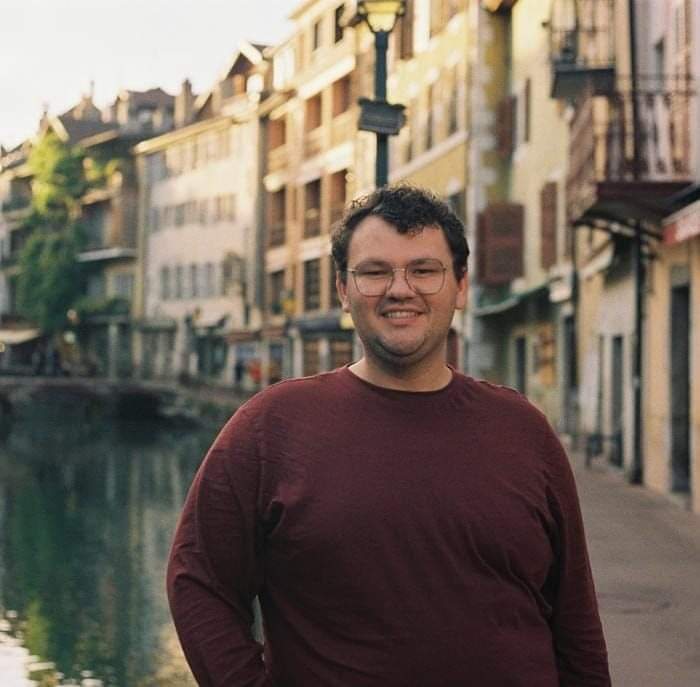
\includegraphics[width=0.9\linewidth]{figs/Gill_2022.jpg} % Replace with your image file
        \end{center}
        \columnbreak
        \begin{description}[font=\bfseries]
            \item[Name:] Ty Gill-Saucier
            \item[Contact:] \href{mailto:ztgill@uw.edu}{ztgill@uw.edu}
            \item[Research Interests:] Sociophonetics, Language
            Ideologies, Mississippi Gulf Coast French, Phonetic bias in
            Automated Speech Recognition (ASR).
        \end{description}
    \end{multicols}
\end{frame}

%-----------------------------------------------------------
\section{Course goals}
%-----------------------------------------------------------
\begin{frame}{Course Goals}
    At the end of this course, you should be able to:
    \begin{enumerate}
        \item \textbf{Articulatory description and understanding}: how sounds of the worlds languages are articulated
        \item \textbf{Practical phonetic competence}: perceive and produce many of the world’s speech sounds
        \item \textbf{IPA transcription}: learn the International Phonetic Alphabet, a universal system for transcribing speech sounds
    \end{enumerate}
\end{frame}

%-----------------------------------------------------------
\section{DRS Accommodations}
%-----------------------------------------------------------

\begin{frame}{DRS Accommodations}
    \begin{itemize}

        \item If you have a disability and may require accommodations to fully participate in this class, please visit the Disability Resources for Students (DRS) website at \url{https://disability.uw.edu/}.
        \item DRS will work with you and me to make arrangements for accommodations.
    \end{itemize}
\end{frame}

%-----------------------------------------------------------
\section{Course overview}
%-----------------------------------------------------------


\begin{frame}{Course Overview}
    \begin{itemize}
        \item Class meets: Tuesdays and Thursdays, 8:30am - 10:20am
        \item Location: CUM 120
    \end{itemize}
\end{frame}

\begin{frame}{Course Overview}
    \begin{itemize}
        \item Class 
    \end{itemize}
\end{frame}

%-----------------------------------------------------------
\section{Assignments and Grading}
%-----------------------------------------------------------
\begin{frame}{Assignments and Grading}
    \begin{itemize}
        \item
    \end{itemize}
\end{frame}     

\begin{frame}{Assignments and Grading}
    \begin{itemize}
        \item
    \end{itemize}
\end{frame}

%-----------------------------------------------------------
\section{Policies}
%-----------------------------------------------------------
\begin{frame}{Policies}
    \begin{itemize}
        \item
    \end{itemize}
\end{frame}

\begin{frame}{Policies}
    \begin{itemize}
        \item
    \end{itemize}
\end{frame}

%-----------------------------------------------------------

% \appendix
% %-----------------------------------------------------------
% \section<presentation>*{\appendixname}
% %-----------------------------------------------------------
% %-----------------------------------------------------------
% \subsection<presentation>*{References}
% %-----------------------------------------------------------
% \begin{frame}[t,allowframebreaks]
%   \frametitle<presentation>{References}
%     \printbibliography
% \end{frame}

% %-----------------------------------------------------------
% \subsection<presentation>*{Variable Importance}
% %-----------------------------------------------------------
% \begin{frame}
%   \frametitle<presentation>{Variable Importance}

% \end{frame}
\end{document}